\documentclass[a4paper]{article}
\def\DOCTITLE{CSC3223 Graphics for Games}
% Set document attributes
\title{\DOCTITLE}

\usepackage{fullpage}
\usepackage{scrextend}
\usepackage{titlesec}
\usepackage{fancyhdr}
\usepackage{amsmath}
\usepackage{amssymb}
\usepackage[section]{placeins}
\usepackage{booktabs}
\usepackage{hyperref}
\usepackage{tikz}
\usepackage{graphicx}
\usepackage{minted}
\usepackage{subcaption}

% Setup headers and footers
\pagestyle{fancy}
\lhead{}
\chead{\DOCTITLE}
\rhead{}
\rfoot{}
\cfoot{\thepage}
\lfoot{}

% New page for each section
\newcommand{\sectionbreak}{\clearpage}

% Set header and footer sizes
\renewcommand{\headrulewidth}{0.4pt}
\renewcommand{\footrulewidth}{0.4pt}
\setlength{\headheight}{15.2pt}
\setlength{\headsep}{15.2pt}

\setlength{\parskip}{5pt plus 1pt minus 1pt}
\setlength{\parindent}{0pt}

% Newline after paragraph
\newcommand{\Para}[1]{\paragraph{#1}\mbox{}}

% Stuff used in cryptography notes
\newcommand{\Forall}{\;\forall\;}
\newcommand{\Mod}{\: mod \:}

% Stuff used in distributed systems notes
\newcommand{\happenbefore}{\rightarrow}
\newcommand{\orderbefore}{\Rightarrow}
\newcommand{\clockcond}{\leadsto}
\newcommand{\RArrow}{$\rightarrow$}

\def\checkmark{\tikz\fill[scale=0.4](0,.35) -- (.25,0) -- (1,.7) -- (.25,.15) -- cycle;}


\begin{document}

\tableofcontents

\section{Overview}

\subsection{3D Graphics}

\begin{itemize}
  \item Scene made up of objects made up of primitives
  \item Primitives are a collection of vertices
  \item Vertices have attributes (position, colour, texture coordinate, etc.)
\end{itemize}

\subsubsection{Primitives}

\begin{figure}[h]
  \centering

  \begin{subfigure}[b]{0.3\textwidth}
    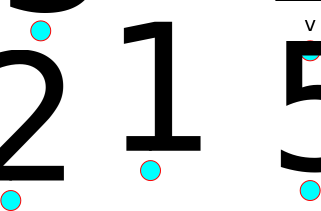
\includegraphics[width=0.8\textwidth]{out/rast_pri_points.eps}
    \caption{Point}
  \end{subfigure}
  \begin{subfigure}[b]{0.3\textwidth}
    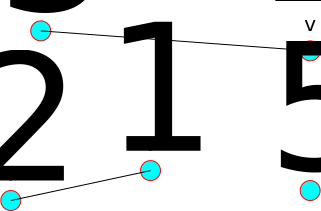
\includegraphics[width=0.8\textwidth]{out/rast_pri_lines.eps}
    \caption{Line}
  \end{subfigure}
  \begin{subfigure}[b]{0.3\textwidth}
    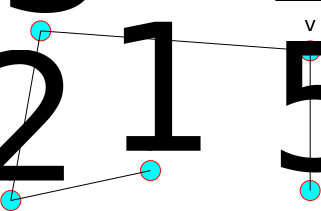
\includegraphics[width=0.8\textwidth]{out/rast_pri_line_strip.eps}
    \caption{Line Strip}
  \end{subfigure}

  \vspace{2em}

  \begin{subfigure}[b]{0.3\textwidth}
    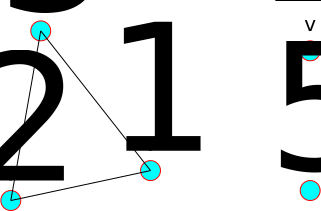
\includegraphics[width=0.8\textwidth]{out/rast_pri_triangle.eps}
    \caption{Triangle}
  \end{subfigure}
  \begin{subfigure}[b]{0.3\textwidth}
    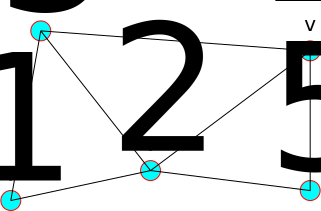
\includegraphics[width=0.8\textwidth]{out/rast_pri_triangle_strip.eps}
    \caption{Triangle Strip}
  \end{subfigure}
  \begin{subfigure}[b]{0.3\textwidth}
    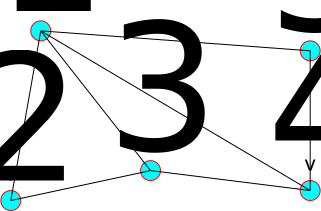
\includegraphics[width=0.8\textwidth]{out/rast_pri_triangle_fan.eps}
    \caption{Triangle Fan}
  \end{subfigure}

  \caption{}
  \label{fig:primitives}
\end{figure}
\FloatBarrier

\subsection{Graphics Pipeline}

\begin{figure}[h!]
  \centering
  \includegraphics[width=0.6\textwidth]{out/graphic_pipeline.eps}
  \caption{Pipeline}
  \label{fig:graphics_pipeline}
\end{figure}
\FloatBarrier

\subsubsection{Vertex Operations}

\begin{enumerate}
  \item[1] Vertices are transformed through a number of matrix operations
           (section \ref{sec:transformations})
  \item[2] Primitives outside screen space are removed (culled)
  \item[3] Vertices outside the screen space are clipped
  \item[4] 3D scene is projected onto a 2D plane
\end{enumerate}

\subsubsection{Fragment Operations}

\begin{enumerate}
  \item[1] Once screen area for a primitive is determined it is rasterised
           (section \ref{sec:rasterisation})
  \item[2] Each fragment is then shaded depending on colour, texture, lighting,
           etc.
\end{enumerate}

\section{Rasterisation}
\label{sec:rasterisation}

\subsection{Line}

Rasterise using Bresenham's line algorithm.

Very simple and fast algorithm for rasterising a line given two 2D points
$(x_{0}, y_{0})$ and $(x_{1}, y_{1})$.

\begin{enumerate}
  \item[1]
    Determine if the line is steep or shallow with respect to the $x$ axis \\
    A steep line is closer being parallel with the $y$ axis

  \item[2]
    Calculate gradient $m = \delta y / \delta x = (y_{1} - y_{0}) / (x_{1} -
    x_{0})$

  \item[3]
    Iterate over the scan (longer) axis \\
    Maintain coordinates of current pixel and $error$ variable

    \begin{enumerate}
      \item[i]
        Shade pixel at current coordinates

      \item[ii]
        Increment the scan axis of current coordinate

      \item[iii]
        $error = error + m$

      \item[iv]
        If $error \geq 0.5$ then increment the periodic axis of current coordinate
        and set $error = error - 1$

    \end{enumerate}

\end{enumerate}

\subsection{Triangle}

\begin{enumerate}
  \item[1] Compute bounding box around triangle
  \item[2] Iterate through each pixel of each line
  \item[3] If the pixel is inside the triangle then shade it
\end{enumerate}

Two common methods for determining if a point is inside a triangle.

Both based on the creation of a temporary vertex $p$ with coordinates of the
pixel being tested.

\subsubsection{Line Equation method}

\begin{enumerate}
  \item[1] Extend lines out from $p$ to each edge of the triangle that are
           perpendicular to the edge
  \item[2] When the direction of each line is towards $p$, $p$ is inside the
           triangle if the distance of each line is positive
\end{enumerate}

\begin{figure}[h]
  \centering
  \begin{subfigure}[b]{0.48\textwidth}
    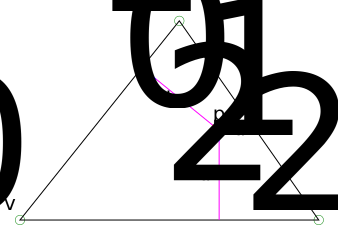
\includegraphics[width=0.8\textwidth]{out/tri_lineeq_in.eps}
    \caption{Inside triangle}
  \end{subfigure}
  \begin{subfigure}[b]{0.48\textwidth}
    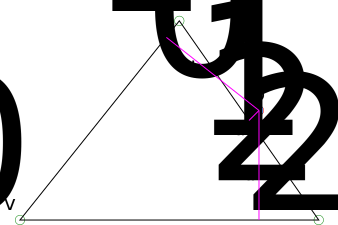
\includegraphics[width=0.8\textwidth]{out/tri_lineeq_out.eps}
    \caption{Outside triangle ($d_{1} < 0$)}
  \end{subfigure}
  \caption{}
  \label{fig:tri_lineeq}
\end{figure}
\FloatBarrier

\subsubsection{Barycentric Coordinate method}
\label{sec:barycentric}

\begin{enumerate}
  \item[1] Create three new triangles ($t_{0}$, $t_{1}$ and $t_{2}$) using $p$
           and vertices of triangle
  \item[2] Calculate area of sub triangles as a proportion of the area of the
           original triangle (using shoelace formula)
  \item[3] If sum of areas of sub triangles $\sum_{i} t_{i} = 1$ then $p$ is
           inside triangle
\end{enumerate}

\begin{figure}[h]
  \centering
  \begin{subfigure}[b]{0.48\textwidth}
    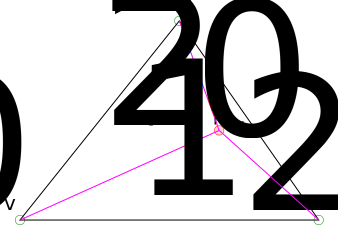
\includegraphics[width=0.8\textwidth]{out/tri_bary_in.eps}
    \caption{Inside triangle}
  \end{subfigure}
  \begin{subfigure}[b]{0.48\textwidth}
    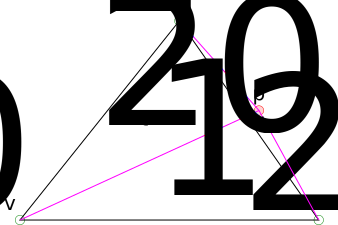
\includegraphics[width=0.8\textwidth]{out/tri_bary_out.eps}
    \caption{Outside triangle}
  \end{subfigure}
  \caption{}
  \label{fig:tri_bary}
\end{figure}
\FloatBarrier

Barycentric areas typically denoted as $\alpha$, $\beta$ and $\gamma$.

\subsubsection{Shoelace formula}

Method of calculating area of any 2D non self-intersecting polygon.

\begin{enumerate}
  \item[1] Create a matrix of the vertices in a closed loop
  \item[2] Multiply the first set of stepped pairs ($s_{1}$)
  \item[3] Multiply the second set of stepped pairs ($s_{2}$)
  \item[4] Calculate area $a = (s_{1}- s_{2}) / 2$
\end{enumerate}

\begin{figure}[h!]
  \centering
  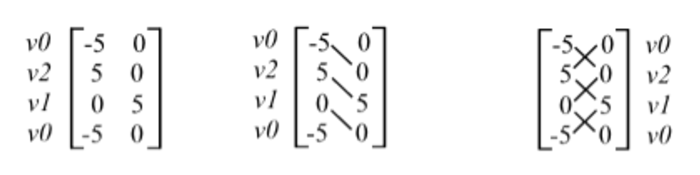
\includegraphics[width=0.6\textwidth]{graphics/shoelace_formula.eps}
  \caption{Shoelace formula example}
  \label{fig:shoelace_formula}
\end{figure}
\FloatBarrier

\subsubsection{Triangle spans}

Triangles can also be rendered using spans, where it is made up of several
lines.

Span start and end points are obtained using the lines between vertices $v_{0}$
and $v_{1}$ (start) and $v_{2}$ and $v_{1}$ (end).

\begin{figure}[h!]
  \centering
  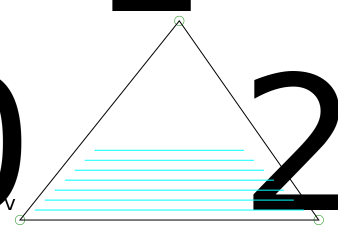
\includegraphics[width=0.6\textwidth]{out/tri_spans.eps}
  \caption{Triangle spans}
  \label{fig:tri_spans}
\end{figure}
\FloatBarrier

\section{Transformations}
\label{sec:transformations}

\subsection{Spaces}

\begin{description}
  \item[World] \hfill \\
    3D space containing everything

  \item[Camera] \hfill \\
    3D space containing the view from the camera \\
    Origin is camera position \\
    Obtained through camera transform

  \item[Clip] \hfill \\
    Only the primitives that can be seen by the camera \\
    Obtained through perspective transform

  \item[Normalised Device Coordinates] \hfill \\
    Transformed from clip space \\
    Coordinates normalised to 1 for hardware compatibility

  \item[Viewport Coordinates] \hfill \\
    Coordinates on a particular screen

\end{description}

\subsection{Scale}

TODO

\subsection{Translation}

TODO

\subsection{Rotation}

TODO

\section{Fragment Operations}
\label{sec:fragment_operations}

\subsection{Interpolation}

\Para{Lines}

Colour at point $p$ computed through simple linear interpolation between
vertices $v_{0}$ and $v_{1}$.
\begin{align*}
  C_{p} &= (C_{b} * t) + (C_{a} * (1 - t)) \\
      t &= |(v_{1} - p) / (v_{1} - v_{0})|
\end{align*}

\Para{Triangles}

Use Barycentric coordinates (section \ref{sec:barycentric}).
\[
  C_{p} = (\alpha * C_{a}) + (\beta * C_{b}) + (\gamma * C_{c})
\]

\subsection{Transparency}

Transparency denoted by alpha value in colour.

$\alpha = 1$ denotes full opacity, $\alpha = 0$ denotes full transparency.

Colour computed by blend equation:
\[
  C = (C_{source} * F_{source}) + (C_{dest} * F_{dest})
\]

Factors $F_{source}$ and $F_{dest}$ are usually programmable but a common
approach is standard linear blending:
\begin{align*}
  F_{source} &= \alpha \\
    F_{dest} &= 1 - \alpha
\end{align*}

One other alternative is additive blending:
\begin{align*}
  F_{source} &= 1 \\
    F_{dest} &= 1
\end{align*}

\end{document}
